\documentclass[11pt, letterpaper, onecolumn]{article}
 
\usepackage[english]{babel}
\usepackage{soul}
\usepackage{mathtools}
\usepackage[utf8]{inputenc}
\usepackage{graphicx}
\usepackage{float}
\usepackage[german=quotes]{csquotes}
\usepackage{hyperref}
\usepackage{fancyhdr}
\usepackage{gensymb}
\usepackage{units}
\usepackage{hhline}
\usepackage{color}
\usepackage{titling}
\usepackage[normalem]{ulem}
\usepackage[margin=2.5cm]{geometry}
\usepackage{amsmath}
\usepackage{amssymb}
\usepackage{amsfonts}
\usepackage{pgfplots}
\usepackage{array}
\usepackage{makecell}
\usepackage{subfigure}
\usepackage{lipsum}
\usepackage{url}
\usepackage{relsize}

\newgeometry{a4paper, left=20mm, right=20mm, top=30mm, bottom=30mm}
\definecolor{pantone294}{cmyk}{1,0.6,0,0.2}
\setlength{\columnsep}{6mm} 

\title{Project 1: QM point particle in external potential} 
\author{Florian Telleis / Florian Hollants / Mickey Wilke}
\date{\today}

\pagestyle{fancy}
\lfoot{Humboldt-Universität zu Berlin}
\rfoot{Project 1.1} 



\begin{document}
	
	\newgeometry{left=14mm, right=13.5mm, top=13.5mm, bottom=30mm}
	\begin{titlepage}
		\thispagestyle{empty}
		\begin{figure}
			
		\end{figure}
		\vspace*{-43mm}\hspace{-6mm}\textbf{\textcolor{pantone294}{\large{Mathematisch-Naturwissenschaftliche Fakultät}}}\\\\\\\\\\
		\textcolor{pantone294}{Institut für Physik}\\
		\vspace{30mm}
		\begin{center}
			\textcolor{pantone294}{\huge{Computational Physics II}}\\\vspace*{7mm}
			\textcolor{pantone294}{\huge{\textbf{\thetitle}}}\\\vspace*{10mm}
			\textcolor{pantone294}{\theauthor}\\\vspace*{10mm}
			\textcolor{pantone294}{\thedate}\\\vspace*{20mm}
			\begin{tabular}{ll}
				\textbf{Work Group:} & Albert Einstein	 \\ \\
				\textbf{Students:} & Florian Telleis (612716) \\
									& Florian Hollants (------)\\
									& Mickey  Wilke (642815)\\ \\
				\textbf{Submitted:} & --.11.2024 \\ \\				
			\end{tabular}
		\end{center}
	\end{titlepage}
	\makeatother
	\restoregeometry
		
		\newpage
	
	
	
	
	
	
    \tableofcontents
    \vspace{1cm}
    
    
    
    
    
    \section{How the code works}








    

    \section{Tests}



















    \section{Workflow}















    
\section{Results and Interpretations}

\subsection{Test results}
First we tested the hamiltonian for linearity, hermicity and positivity. The maximum error for the linearity and hermicity are around $10^{-13}$ which we put in the realm of floating point errors. We have also shown, that the hamiltonian is always positive semi-definite. Furthermore we tested the eigenvalues and eigenvectors of the hamiltonian for the potential $V=0$ and got a maximum error on the order of $10^{-12}$, which we also count as floating point error, since the calculation for this test carried the error for more operations compared to the other tests, making it bigger.\\
Next we tested both integrators for linearity, unitarity and energy conservation. Both integrators had a maximum error for linearity on the order of $10^{-15}$, which is well into the domain of floating point errors, so just as we expected, both integrators are linear. On the other hand only the Strang-Splitting integrator was unitary, conserving the norm with a maximum error on the order of $10^{-15}$, while the Second-Order integrator is not unitary with a maximum error on the order of $10^{-5}$. This error is way too big to be discounted as a floating point that was carried over after initialization. Lastly neither Second-Order, nor Strang-Splitting conserves energy, with the error being on the order of $10^{-4}$ and $10^{-7}$ respectively.\\
All in all the results of the tests are as we expected, giving some confidence that these functions work as intended.
\subsection{Simulation}
The wave function starts in the vicinity of the left minimum, moving to the right. Approaching the maximum in the middle of the potential, the peak of the wave function lowers and the spread becomes bigger, indicating that the wave function "avoids" areas of high potential energy as intended. Part of the wave function gets past the maximum, while the rest is reflected, and starts moving to the left. The wave function shortly develops some sort of small "discontinuity" at the point where the two halves separate, which is not clear weather it is an artifact of the discretization or is just how the wave function is supposed to split, given the potential. The wave function becomes much less "smooth" when it starts overlapping with high energy regions of the potential on the left and on the right side. This disturbance can most likely be attributed to the discretization effects, but we haven't been able to find initial conditions and parameters that keep the wave function "stable" even after "collision" with the boundary. On the other hand, the potential grows quick enough to prevent the wave function on both sides, of interacting with each other by crossing the boundary of the domain.
\subsection{Scaling and Convergence}
We plotted the Energy of the wave function after M iterations of both the integrators against the value of M as a log-log plot. We were expecting the relationship to be some sort of power law. \\
$E\sim \hat{\tau}^n\sim M^{-n}$\\
In the log log plot we would then see a straight line with slope $-n$. Contrary to that we did not find a straight line over most of the domain. Especially for low values of M the Energy increases drastically. One side effect of the log-log plot is, that the density of points decreases for lower values on the x-axis. On the plot for the Energy of the Second-Order integrator one can clearly see the cut-off point, after which the wave function becomes unstable even during one full time step. The same cut-off can be seen on the graph plotting the norm of the Second-Order integrator, albeit less pronounced.
\begin{figure}[!h]
    \centering
    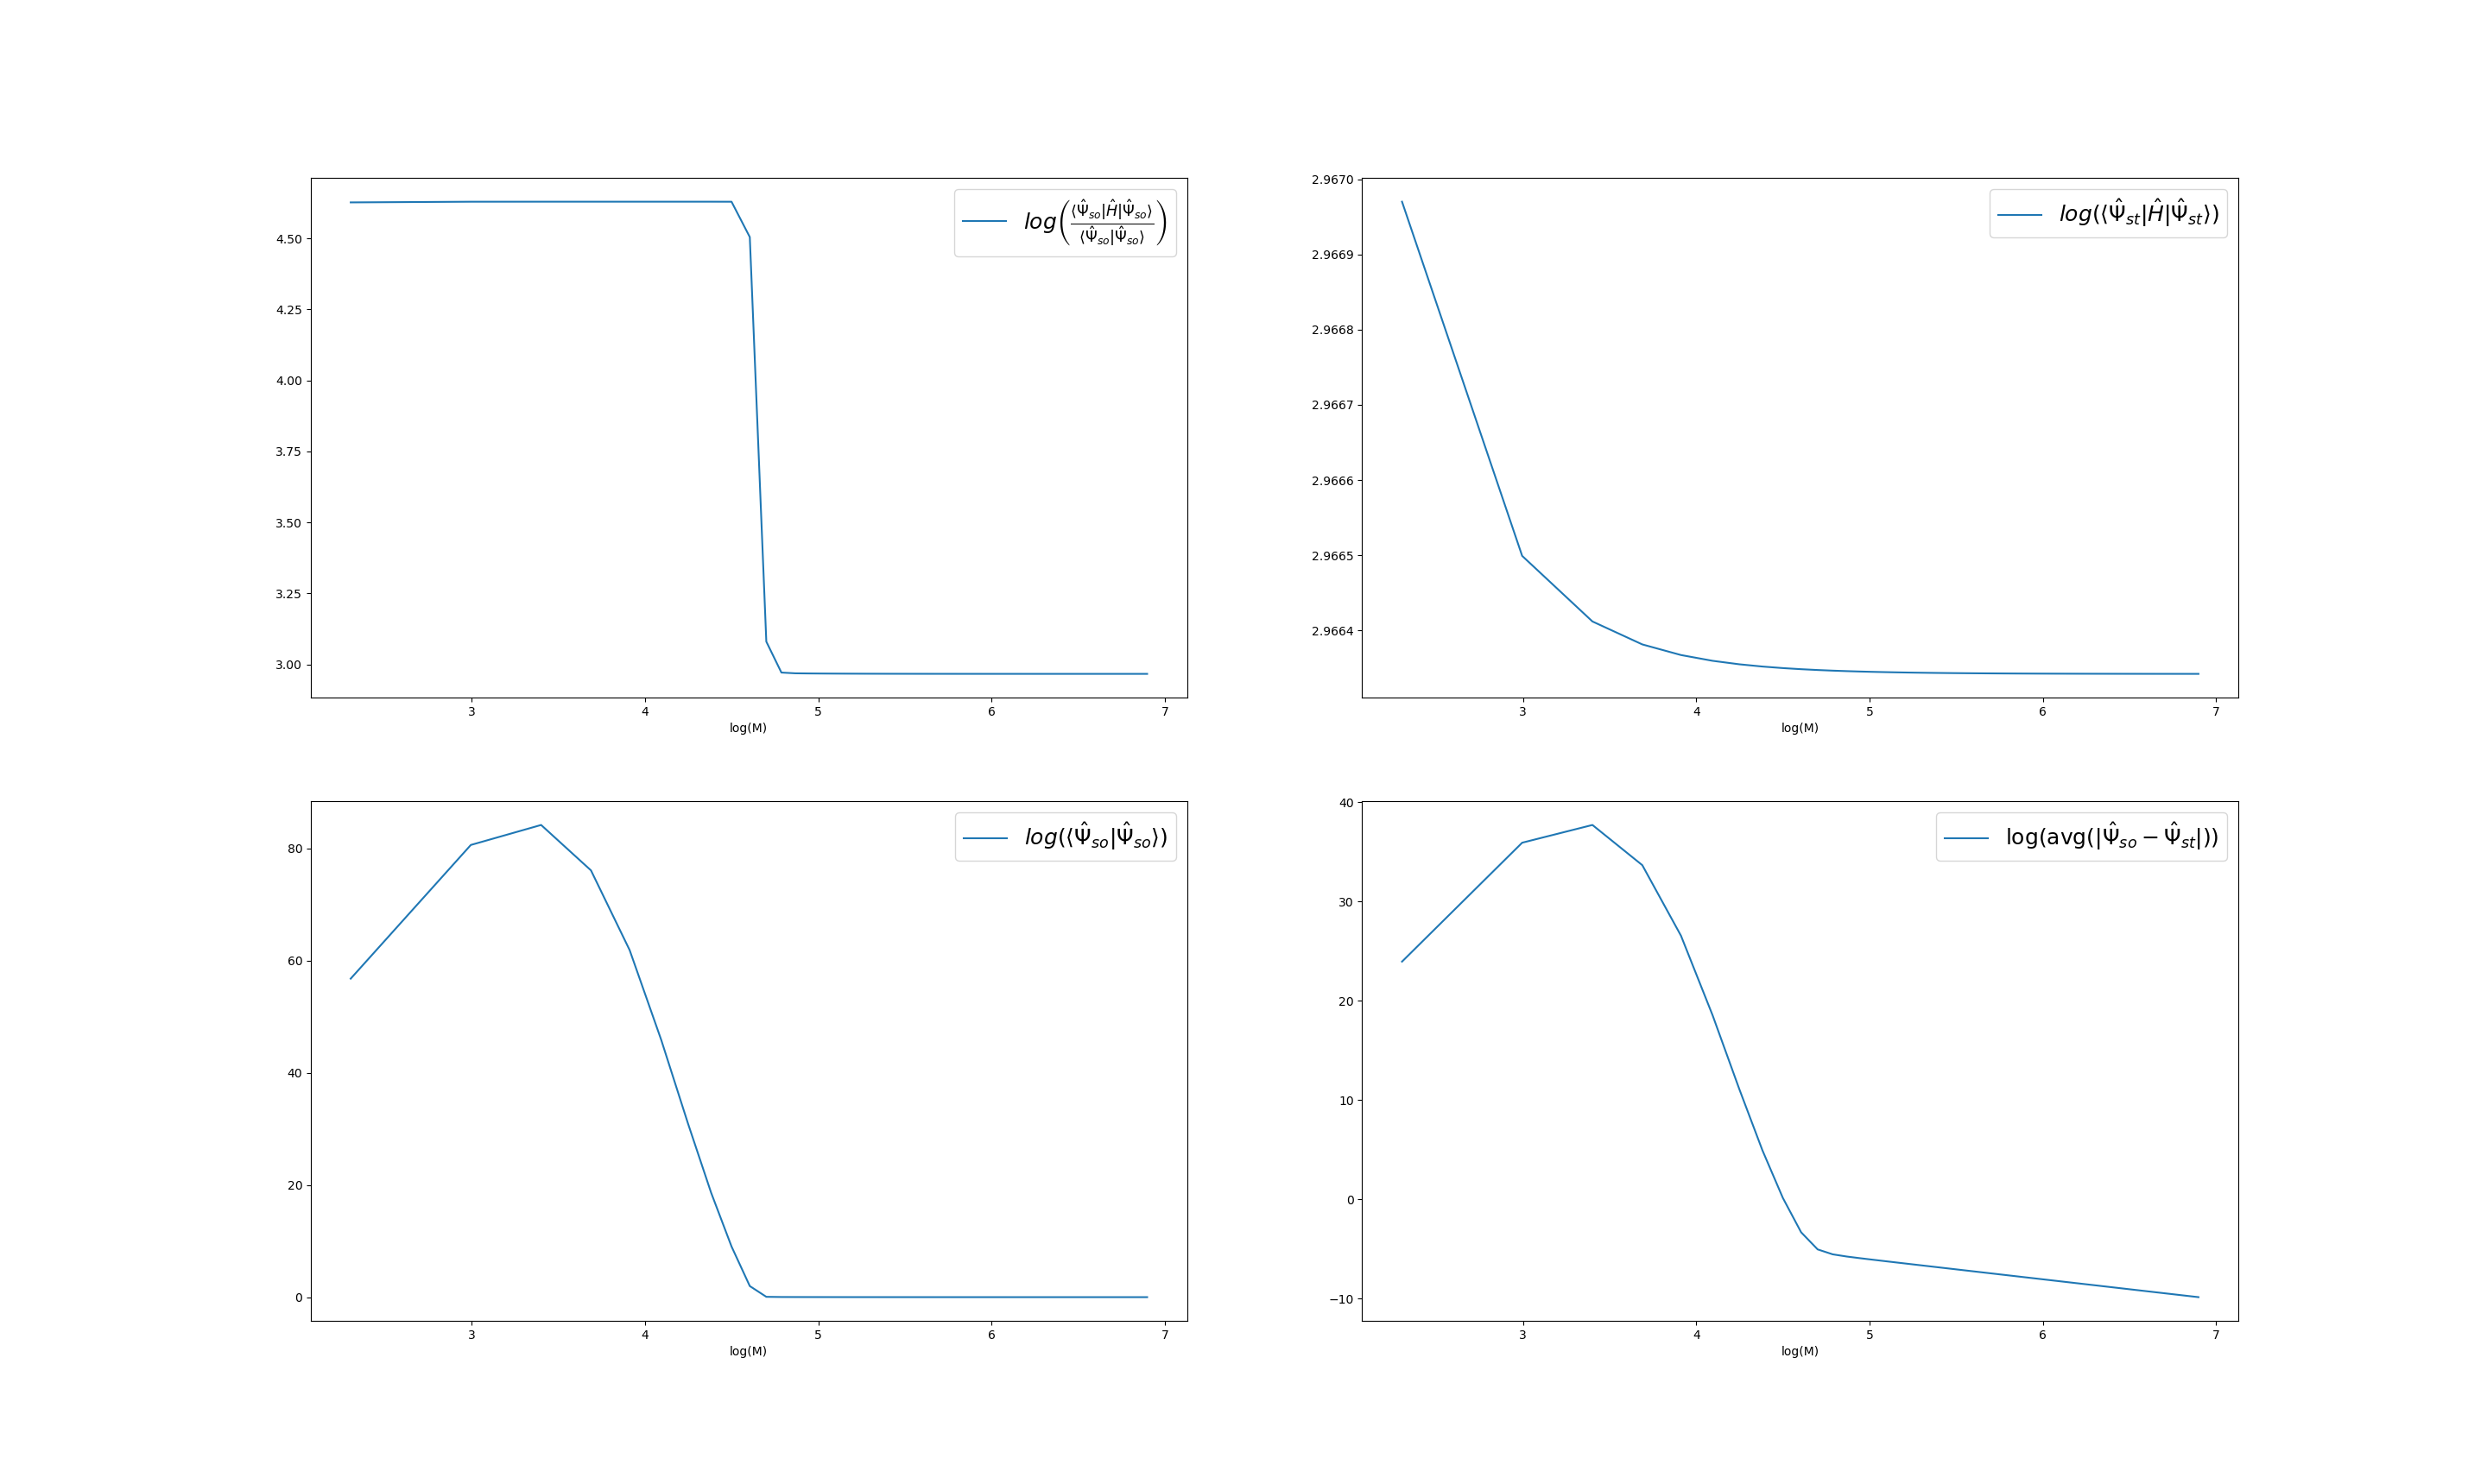
\includegraphics[width=.9\textwidth]{logvlog.png}
    \caption{log-log plot for $M\in[10, 990]$ }
\end{figure}\noindent\newline
When looking at higher values of M we can see the predicted linear plot for the difference between the two integrators implying the relationship $\ket{\Psi_{so}(t)}-\ket{\Psi_{st}(t)}\sim\tau^2$. For the other graphs we were not able to determine the relationship with tau, even for higher values of M.
\begin{figure}[!h]
    \centering
    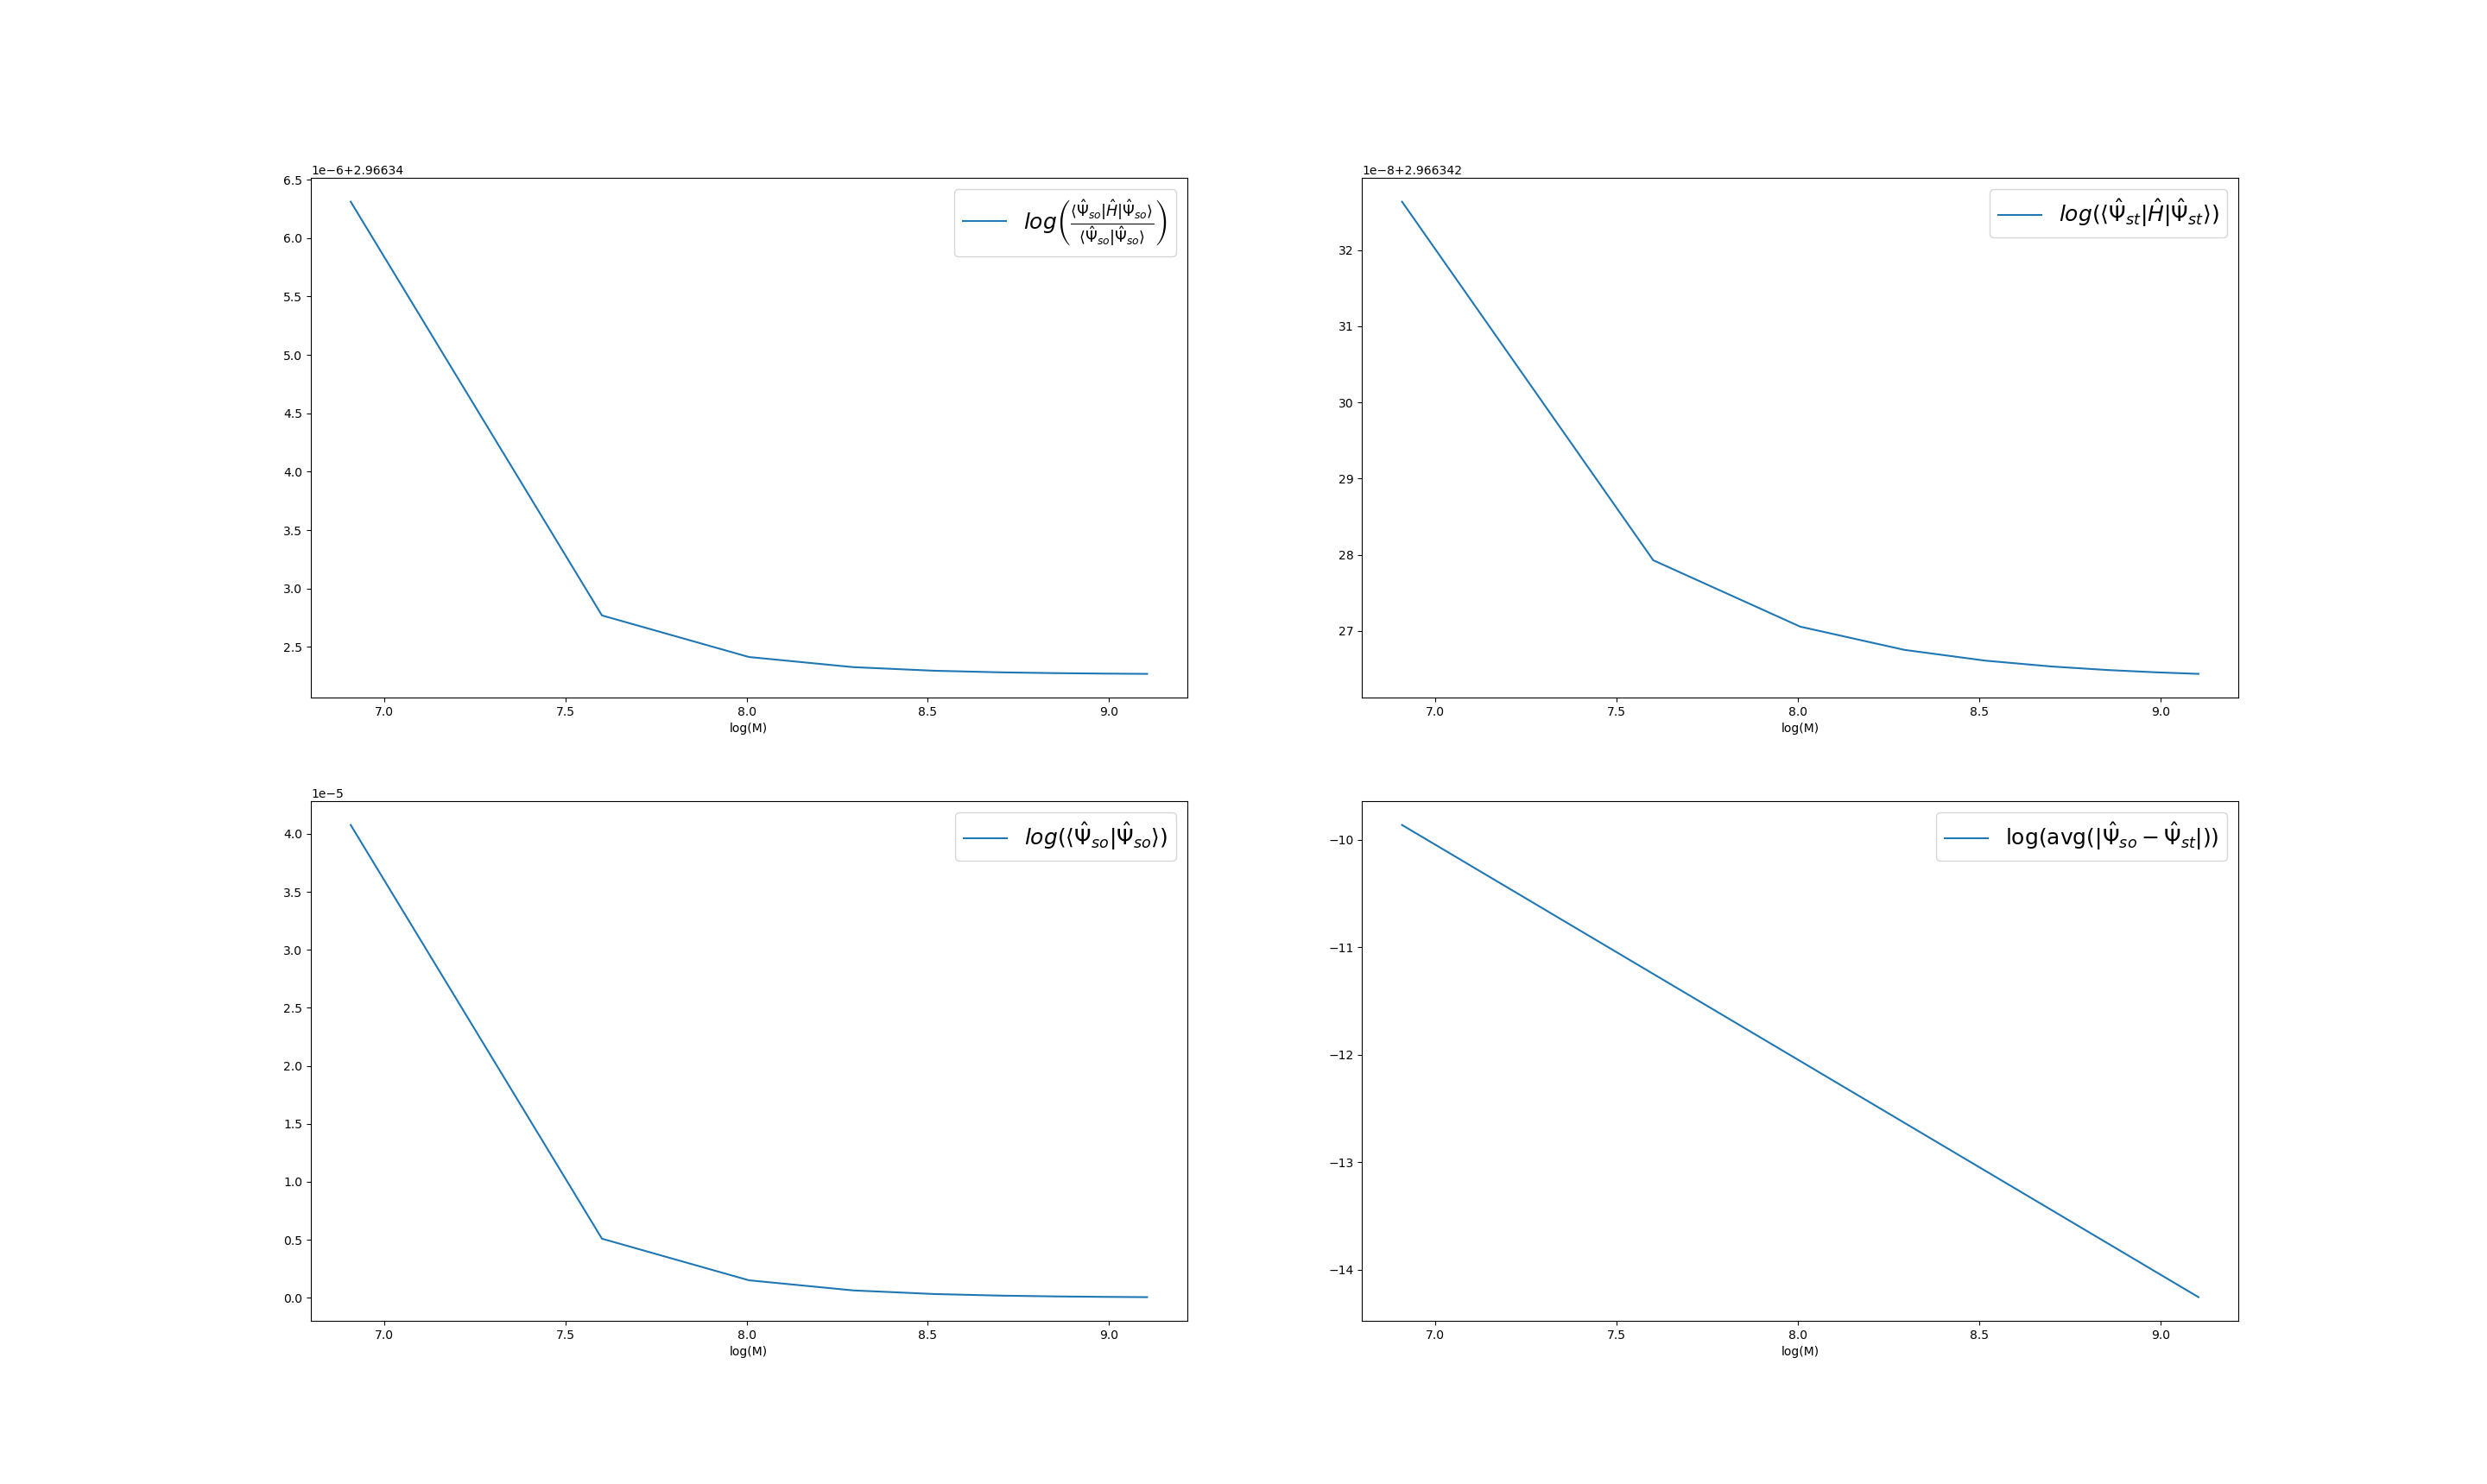
\includegraphics[width=.9\textwidth]{plots_for_1000M9000.png}
    \caption{log-log plot for $M\in[1000, 9000]$ }
\end{figure}\noindent\newline












    
	










	

	
	





	
\end{document}
